\documentclass{article}
\usepackage[a4paper, margin=2cm]{geometry}
\usepackage[utf8]{inputenc}
\usepackage{graphicx}

\begin{document}
\begin{center}
    \Large Building management system\\
    {\large Adam Polický, Jiří Klepl, Martin Gora, Štěpán Stenchlák}
\end{center}

\smallskip{}

The main purpose of this system is to have a locally centralized view and control of the building’s lights, cleaning devices, and thermostats.

\section*{Stakeholders}

\begin{itemize}
\itemsep0em 
\item \textbf{Healthcare personnel} - access to temperature/lights/cleaning-devices settings for their particular department
\item \textbf{Cleaning service} - management and planning of the cleaning-devices, want an intuitive application for cleaning automatization 
\item \textbf{Janitor (building management)} - overview of the whole building, ability to control building appliances
\item \textbf{Technician} - fixes lights, robots; wants overview, has direct access to DB and software services
\item \textbf{IT infrastructure} - they will run the system; they want an overview, logs; they care about the price, development time, stability of the system, and its maintainability    
\item \textbf{Hospital management} - interested in the overall state of the system and hospital buildings
\item \textbf{System owner} - is interested in the price, scalability, and extensibility of the system
\end{itemize}

\section*{Decomposition module viewpoint}

\begin{figure}[h]
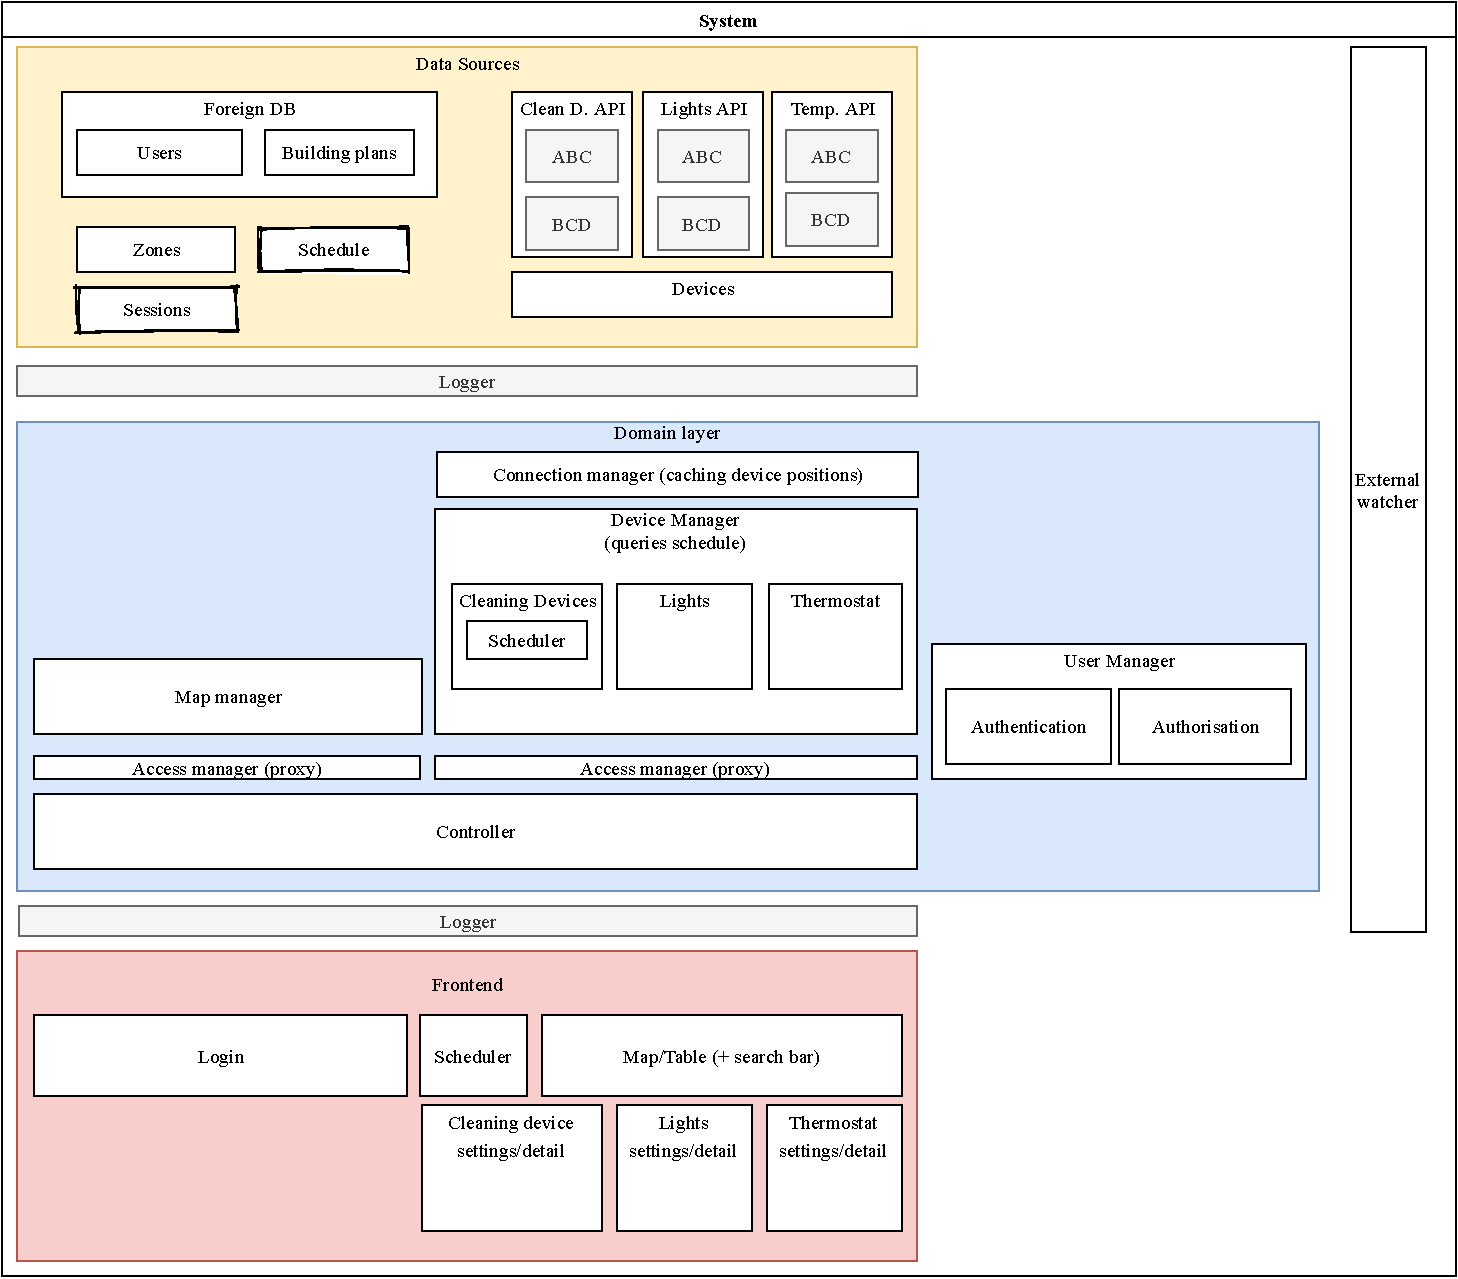
\includegraphics[width=.9\textwidth]{decomposition.pdf}
\centering
\end{figure}

\newpage
\section*{Usage module viewpoint}

\begin{figure}[h]
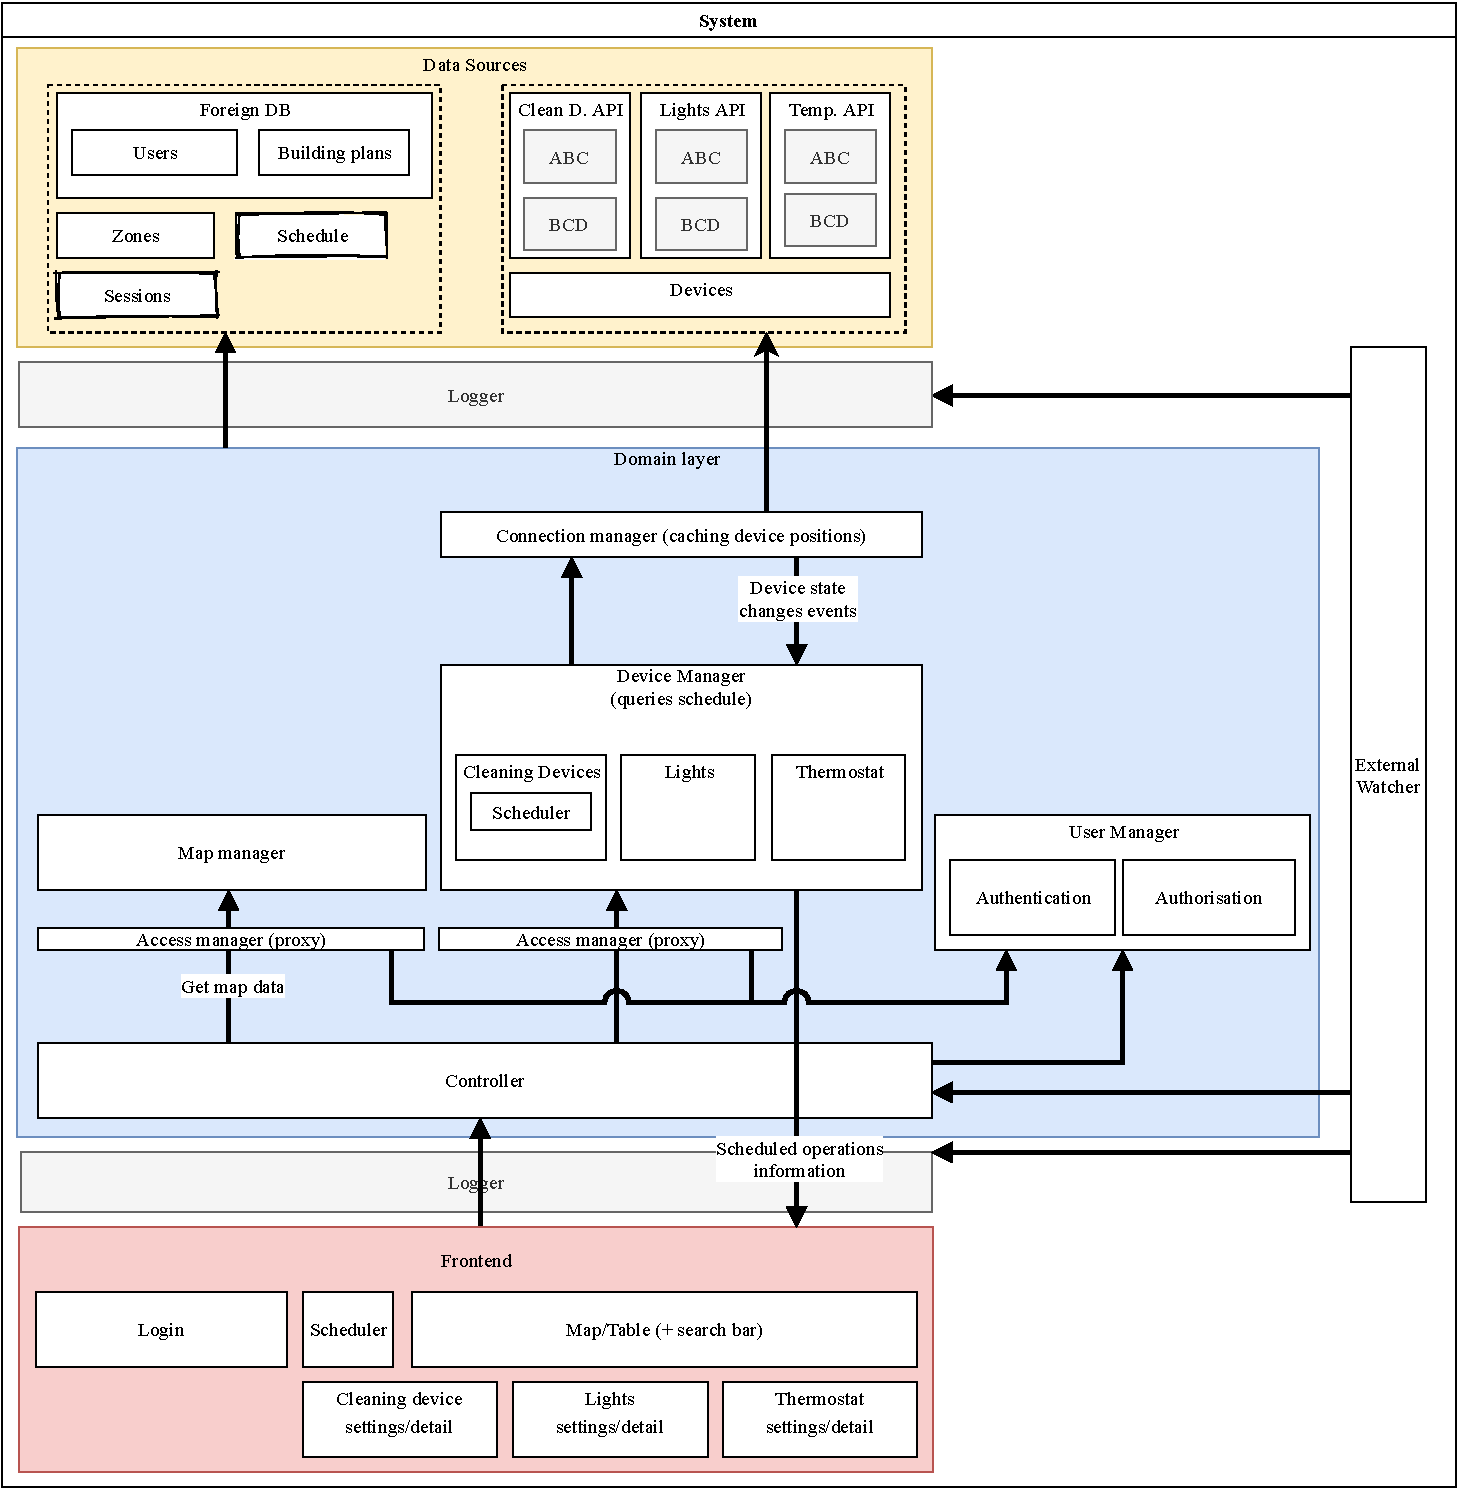
\includegraphics[width=.9\textwidth]{Usage.pdf}
\centering
\end{figure}

\end{document}